\documentclass{eplDoc}

\usepackage{placeins}

\newcommand{\docType}	{Assignment 1 : Markov Decision Processes}
\newcommand{\docDate}	{16/03/2012}
\newcommand{\docAuthor}	{gr10 : Mulders Corentin, Pelsser Francois}
\newcommand{\courseCode}{SINF2275}
\newcommand{\courseName}{Data mining and decision making}
\usepackage{syntax}

\lstset{breaklines=true, breakatwhitespace=false}

\begin{document}
\maketitle
\newpage

\section{Method used to determine the optimal strategy}

\subsection{Brief description of the method}
To select the dice to throw in the current state we use a markov decision process. To do this we had to define a way to represent the problem and implement the markov process itself. 

\subsubsection{Representation of the problem}
We define the state of the game as the number of the square on wich the player is. At each state the only two possible actions are to throw the security or the risky dices. Our actions all have a fixed cost of $1$ independently of the state (this is only true if there are no prison squares, when we add those they lead to some actions having a cost of $2$ as it will be explained later). \\ 
We represent the game board as an affinity matrix, its elements are : 
\begin{itemize}
	\item $a_{ij}=0$ if the player can't move from i to j in one step.
	\item $a_{ij}=1$ if the player goes from i to j following the main path.
	\item $a_{ij}=2$ if the player goes from i to j following a secondary path.
\end{itemize}
The case when the game stops whenever the player goes through the arrival is represented by the affinity matrix arrival going to itself. In other words if g is the goal then $a_{gg} = 1$. \\ 
And if the game is setso that the board is a loop and the player must stop on the arrival to win then if $s$ is the starting point and $g$ the goal $a_{gs} = 1$. \\ \\ 

The initial state and goal state values are also stored each in a variable. \\ 
In addition to this we have the vector List received as argument that defines the types of squares. \\ 

\subsubsection{Markov decision process}
We use the value iteration algorithm to compute the optimal expected cost. 
To do that, we are working in multiple phases.  First we compute probabilities, 
we create 2 matrix (one for each dice) where every element $a_{i,j}$ represents 
the probability to go from the case $i$ to the case $j$ by playing the dice related to the matrix.\\
Computing the first matrix is pretty straightforward.  We first set every $a_{i,i}$ to $0.5$, then we count the number of element bigger than $0$ in the line $i$ and for all theses elements we add a probability of $O.5$ over the number of element. \\
Ex : if the case $1$ is the junction of 2 path and the next cases are $2$ $4$ we have the $i th$ line of the probability matrix that start with : $[0.5\  0.25\ 0\ 0.25\ 0\ 0\ ...]$\\
For the second dice, the principle is the same, except that all values are not $0.5$ but $1/3$ (1/3 for 0,  1/3 divided by the number of path and the case next to the current case in the path and the last third (also divided by the number of paht) for every cases 2 cases away from the current cases in every pahts.)\\
For this dice, we also have to consider traps, this is done just before adding the probability to a case, we check if it is a trap, and if it is, we add this probability to the case where the trap leads us instead.\\
Then we compute the costs.  Costs for the first dice are always 1 but for de risky dice the cost is set to 2 for the cases with a prison.\\
Then we apply the iteration algorithm and we stop when the absolute value of the difference of the norm of the vector V and the norm of the old vector V is below a threshold (we use $10^-5$).\\
After that we can compute the policy and return it.





\subsection{Additional experiments}


\subsubsection{Prison squares}

If a case is a prison square and the player stops on it when using the risky dice then the cost of the action is $2$ instead of $1$. This is because the consequence sof stopping on such a case is that a turn will be lost. So we can consider that to go on the case we need to throw the dice twice instead of once. 

\subsubsection{retreat squares}

If a case $i$ is a retreat square then, if there is a probability $p$ to stop on this case,  the probability to stop on this case becomes $0$ and there is a probability $p$ to get on the  $i-2$ square (or square $1$ if $(i-2)<1$). Off course that is only the cas eif the dice played was the risky dice. 


\subsubsection{Adaptation to any kind of of Snakes and ladders game}

Since the game board is represented as an affinity matrix it is very easy to use our implementation to play on a different board. The only thing to do is to define the affinity matrix corresponding to the new game and fetch it to the program. Off course the vectors of the traps types must also be adapted to match the number of squares in the game. \\ 
As an example of this functionality we designed a more complex game board and used it with our program. A representation of this new game board is shown below (arrows with interrupted lines represent secondary paths): 

\FloatBarrier
\begin{figure}%
	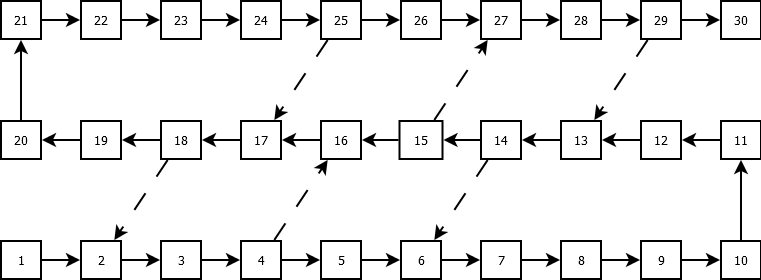
\includegraphics[width=\columnwidth]{newboard.png}%
	\caption{Complex board}%
	\label{newboard}%
\end{figure}
\FloatBarrier
 \ \\ 
%This board will be used as well as the basic board for the analisys of our results compared to a naive strategy. 

%\subsubsection{Use of reinforcement learning}
Custom boards can be passed as parameters to our "snake.m" implementation of the markov decision process. The \textbf{[Expec, Dice] = markovDec(list)} function simply calls "snake.m" with the basic board. 

\section{Results obtained with our implementation}

We used octave to write our implementation of \textbf{[Expec, Dice] = markovDec(list)}. We compare our decision process with three naive policies :
 
\begin{description}
	\item[Security] always plays the security dice.
	\item[Risky] always plays the risky dice.
	\item[Random] has a $50\%$ probability to play either of the dices.
\end{description}
 
We test each of these policies on three different boards. The two first are the variants of the basic board from the assignment instructions. The first one when the game stops whenever a player goes through the arrival square, we will call it the \textbf{simpleBoard1}. And the second one when the game only stops if the player stops on the arrival, we will call it the \textbf{simpleBoard2}. \\ 
The third board used is our example of complex board represented in figure \ref{newboard}, we will call it the \textbf{complexBoard}. \\ \\ 
For each of these boards we used differents traps sets. And for each trap set we simulated 50 games to collect statistics. \\ \\ 

Here are the number of turns needed to finish for the \textbf{simpleBoard1} : 


\begin{center}
		\begin{tabular}{|r|ccc|}
			\hline
			policy & minimum & maximum & mean \\ 
			\hline
			 Security & 8.0000 &  46.0000 &  17.5000 \\
     	Risky & 5.0000  & 42.0000  & 12.4800 \\ 
    	Random & 4.0000 &  49.0000  & 14.2000 \\ 
   		markovDec & 5.0000 &  20.0000 &  10.6800 \\ 
   		\hline
		\end{tabular}
\end{center}


Here are the number of turns needed to finish for the \textbf{simpleBoard2} : 


\begin{center}
		\begin{tabular}{|r|ccc|}
			\hline
			policy & minimum & maximum & mean \\ 
			\hline
			 Security &     9.0000  & 28.0000  & 16.8800 \\
    Risky & 4.0000  & 78.0000 &  18.4200 \\ 
    Random & 5.0000  & 84.0000 &  27.5400 \\ 
    markovDec & 4.0000 &  26.0000  & 11.2000  \\ 
   		\hline
		\end{tabular}
\end{center}

Here are the number of turns needed to finish for the \textbf{complexBoard} : 


\begin{center}
		\begin{tabular}{|r|ccc|}
			\hline
			policy & minimum & maximum & mean \\ 
			\hline
			 Security &                            24          &             788         &           154.78 \\
       Risky &               1001           &           1001          &            1001 \\ 
       Random &               1001        &             1001             &         1001 \\ 
       markovDec &                 17         &              249             &         62.6 \\ 
 
   		\hline
		\end{tabular}
\end{center}

As we can see our markov decision process yields better mean results on every board. However the improvement is most visible on our complex board where the risky and random policies are very bad (the $1001$ number of turns means our program stoped playing without reaching the goal sinc eit took too much turns) and our policy is still nearly two times better than the default security strategy. 




\end{document}
